\documentclass[12pt]{article}

\usepackage[utf8]{inputenc}
\usepackage[T1]{fontenc}
\usepackage[top=2cm, bottom=2cm, left=2.5cm, right=2.5cm]{geometry}
\usepackage{graphicx}
\usepackage{nomencl}
\usepackage{listings}
\usepackage{biblatex}
\usepackage{amsfonts}
\usepackage{hyperref}
\usepackage{float}

\usepackage{subcaption}
\usepackage{tabularx}
\newcolumntype{C}{>{\centering\arraybackslash}X}


\newbibmacro*{bbx:parunit}{%
  \ifbibliography
    {\setunit{\bibpagerefpunct}\newblock
     \usebibmacro{pageref}%
     \clearlist{pageref}%
     \setunit{\adddot\par\nobreak}}
    {}}

\renewbibmacro*{doi+eprint+url}{%
  \usebibmacro{bbx:parunit}% Added
  \iftoggle{bbx:doi}
    {\printfield{doi}}
    {}%
  \iftoggle{bbx:eprint}
    {\usebibmacro{eprint}}
    {}%
  \iftoggle{bbx:url}
    {\usebibmacro{url+urldate}}
    {}}

\renewbibmacro*{eprint}{%
  \usebibmacro{bbx:parunit}% Added
  \iffieldundef{eprinttype}
    {\printfield{eprint}}
    {\printfield[eprint:\strfield{eprinttype}]{eprint}}}

\renewbibmacro*{url+urldate}{%
  \usebibmacro{bbx:parunit}% Added
  \printfield{url}%
  \iffieldundef{urlyear}
    {}
    {\setunit*{\addspace}%
     \printtext[urldate]{\printurldate}}}

\sloppy

\title{Estimating Feature Importance in LSTM-Based Time Series Forecasting via Multi-Objective Evolutionary Optimization: A Reproducibility Study}
\author{Niebo Zhang Ye, Joan Lapeyra Amat, Andreja Andrejic, Rosen Dimov}
\date{Algorithmics for Data Mining, Master in Innovation and Research in Informatics - Universitat Politècnica de Catalunya }

\addbibresource{references.bib}

\begin{document}

\maketitle

\maketitle

\begin{abstract}
Feature selection is a crucial step in time series forecasting, particularly for complex models such as Long Short-Term Memory (LSTM) networks. Recent work has introduced embedded feature selection methods based on multi-objective evolutionary algorithms (MOEAs), enabling simultaneous optimization of LSTM weights and input feature subsets, with feature importance derived from model selection frequency. In this project, our objective is to reproduce and adapt the methodology proposed by Espinosa et al. to estimate the importance of features in LSTM-based time series models. Our approach leverages a multi-objective evolutionary strategy to generate a diverse ensemble of LSTM models trained on different feature subsets, followed by stacking-based ensemble learning. Feature importance is quantified by the frequency of feature selection across the Pareto-optimal models. Due to the complexity of the original algorithm, several simplifications and modifications were introduced in our implementation. We present our methodological adaptations, discuss challenges encountered in reproducing the state-of-the-art, and report experimental results on the Hugging Face dataset electricity demand. Our findings offer practical insights into the feasibility of embedded feature selection for LSTM forecasting and highlight key considerations for future reproducibility and interpretability research.
\end{abstract}

\begin{flushleft}
\end{flushleft}

\begin{flushleft}
Key words:\textbf{ Time Series Forecasting, Feature Selection, LSTM, MOEA, Embedded Feature Selection, Feature Importance Estimation }
\end{flushleft}

\section{Introduction}

Time series forecasting is a fundamental task in machine learning, underpinning applications in domains ranging from finance to environmental monitoring. Accurately predicting future values from sequential data requires models that can capture both short- and long-term dependencies, with Long Short-Term Memory (LSTM) networks emerging as a powerful solution due to their architecture, which effectively mitigates the vanishing gradient problem common in traditional recurrent neural networks.

However, the performance and interpretability of LSTM-based forecasting models are heavily influenced by the quality of the input features. Feature selection (FS) techniques aim to identify a subset of relevant variables, thereby reducing overfitting, improving generalization, and enhancing model transparency. FS methods can generally be classified as filter, wrapper, or embedded approaches. ~\cite{espinosa2023embeddedfeatureselectionlstm} While filter and wrapper methods select features independently of model training or through external evaluation loops, embedded methods integrate feature selection within the training process itself, potentially offering a better balance between accuracy and computational efficiency.

A notable challenge in time-series feature selection is quantifying the relative importance of input features in complex, non-linear models like LSTMs. Recent advances have explored attention mechanisms, sensitivity analysis, and evolutionary algorithms for embedded feature selection, yet robust methods for interpretable and generalizable feature importance remain an open problem, particularly for high-dimensional or multivariate time series~\cite{espinosa2023embeddedfeatureselectionlstm}.

In this work, we investigate the problem of feature importance estimation in LSTM-based time-series forecasting models. Inspired by the embedded feature selection framework proposed by Espinosa et al. ~\cite{espinosa2023embeddedfeatureselectionlstm}, which leverages multi-objective evolutionary algorithms (MOEAs) to simultaneously optimize LSTM weights and feature subsets, we attempt to reproduce and adapt this methodology for our own experimental setting. The referenced approach frames feature selection and model training as a multi-objective optimization task, with ensemble learning used to aggregate the predictive performance of non-dominated LSTM models. Feature importance is then determined by the frequency with which features are selected across the Pareto front.

While we adopted the core concepts of this framework, our implementation involved several adaptations and simplifications due to the complexity of the original method and computational constraints. In particular, certain algorithmic details or experimental procedures could not be exactly matched; these deviations are discussed in Section~\ref{sec:methods}.

Our contributions are as follows:
\begin{itemize}
    \item We provide a practical implementation and empirical evaluation of a feature importance estimation pipeline for LSTM-based time-series forecasting, rooted in multi-objective evolutionary optimization.
    \item We assess the impact of feature selection frequency as a measure of importance in ensemble LSTM models.
    \item We discuss the methodological challenges encountered in reproducing the state-of-the-art, providing insights for future research and open-source implementations.
\end{itemize}

The rest of this paper is organised as follows: Section~\ref{sec:related_work} reviews related work in time-series feature selection and ensemble learning for LSTMs. Section~\ref{sec:methods} details our adopted methodology and any deviations from the original algorithm. Section~\ref{sec:experiments} presents our experimental results using the Hugging Face electricity demand dataset. Finally, Section~\ref{sec:conclusion} concludes the paper and outlines directions for future research.



\section{Related Work}
Working with time series data involves considering peculiarities that are not present in non-temporal datasets. Thus, a lot of Data Mining algorithms have to be modified to be able to accommodate temporal datasets. Even though there has been a lot of research done in the field of feature weighting and feature selection, only a fraction of the work has been towards time series data. A paper relevant to both our problem and our dataset is ~\cite{GONZALEZVIDAL201971} by González-Vidal et al. In this paper, they combine different search strategies with different feature selection algorithms to find the feature subset with the best prediction result. They concurred that the multivariate wrapper feature selection algorithms along with Multi Objective Evolutionary Search gave the best result. Another idea was proposed by Ircio et al in ~\cite{IRCIO2020107525}. Their approach is more mathematical, in that they used Mutual Information (MI). They leveraged MI between all pairs of explanatory features (1), between all features and the target variable (2) and conditional MI between all pairs of explanatory features (3). However, we wanted to use our interest and familiarity with LSTMs, so we strayed away from these research.

\nomenclature[S]{$a^{(l)}$}{ $a^{(l)} = \sigma^{(l)} (z^{(l)})$ activation vector of layer $l$.}
\nomenclature[S]{$z^{(l)}$}{$z^{(l)} = W^{(l)}a^{(l-1)} + b^{(l)}$, pre-activation vector at layer 
$l$.} 
\nomenclature[S]{$W^{(l)}$}{Weights of layer $l$.}
\nomenclature[S]{$b^{(l)}$}{Bias of layer $l$.}
\nomenclature[S]{$f$}{$f\colon \mathbb{R}^n \to \mathbb{R}^m$, function representing the neural network.}
\nomenclature[S]{$m$}{Size of the predicted date / output of the network.}
\nomenclature[S]{$n$}{Size of the input data.}
\nomenclature[S]{$y$}{Target data.}
\nomenclature[S]{$x$}{Input data.}
\nomenclature[S]{$C$}{Loss (cost) function, scalar-value function $C(a^{(l)}, y)$.}
\nomenclature[S]{$\delta^{(l)}$}{Error signal at layer $l$, defined as $\delta^{(l)}_i=\frac{\partial C}{\partial z^{(l)}_i}$.}
 
\section{Methods}
\label{sec:methods}

\subsection{Overview}

Our methodological approach was inspired by Espinosa et al. \cite{espinosa2023embeddedfeatureselectionlstm}, who introduced an embedded feature selection framework for LSTM networks using multi-objective evolutionary algorithms (MOEAs) and ensemble learning. The core idea is to jointly optimize input feature subsets and LSTM parameters, generating a Pareto front of diverse models whose selection frequencies provide an interpretable measure of feature importance. Our implementation adapts and simplifies this methodology to accommodate computational constraints and codebase feasibility, while retaining the essential research questions regarding feature importance estimation in LSTM-based time series forecasting.

\subsection{Data Preprocessing and Partitioning}

As a first approach, the Hugging Face platform provided two separate datasets: weather information and electricity demand data. The time intervals between the two datasets were different, the weather data was recorded hourly, while the electricity demand data was available at 15-minute intervals. To align the datasets, a rolling operation was applied to the demand data to match the hourly weather time window. Additionally, some missing intervals were identified in the dataset, such as 2015, for which no data were available. Consequently, we focused our study on the period from 2016 to 2018.

The data preprocessing pipeline involves removing outlier from the data, normalization of input features and chronological splitting of the dataset. Following the methodology in \cite{espinosa2023embeddedfeatureselectionlstm}, we independently normalize the training and test sets using MinMax scaling to prevent information leakage. The preprocessed dataset is then partitioned into $n$ consecutive, non-overlapping subsets for use in multi-objective optimization; each partition corresponds to a separate objective in the MOEA. All splits and normalization procedures are performed strictly chronologically to preserve temporal structure, in line with best practices for time-series forecasting.

Apart from the data preprocessing pipeline, we included a data augmentation where we extract temporal features from our time series. Aside from the importance of the temporal continuity of the data in time series, many temporal characteristics are lost when we input the data. For example, the hour can be an essential factor in demand, as consumption is clearly lower at night. However, this is not reflected in our current data. Therefore, we have decided to extract some static features. In our specific case, we have used the hour, the day of the week, and the season as static features.

\subsection{Embedded Feature Selection with MOEA}

\subsubsection{Optimization Problem Formulation}

The feature selection and model parameter optimization are jointly formulated as a multi-objective problem. Each solution (individual) in the population is encoded as a concatenation of a binary feature mask (indicating selected input features) and real-valued LSTM weights and biases. The objectives are to minimize the root mean squared error (RMSE) on each of the $n$ data partitions and, optionally, to minimize the number of selected features as a proxy for model sparsity.

\subsubsection{Evolutionary Algorithm}

We employ the NSGA-II algorithm \cite{Miyandoab_2023} as implemented in the Platypus Python library, utilizing mixed binary-real encodings and standard crossover and mutation operators for each type. The fitness of each individual is evaluated by applying the corresponding LSTM, parameterized by the decoded weights and selected features, to each data partition and computing the RMSE. Solutions with zero features selected are penalized to avoid degenerate cases.

The principal advantage of this approach is that it enables simultaneous exploration of both model parameters and feature subsets without reliance on gradient-based optimization, potentially overcoming local minima and discovering sparse, high-performing models. However, the computational cost is substantial, as each fitness evaluation requires a full forward pass of an LSTM on a data partition, and evolutionary search is inherently less sample-efficient than gradient descent.

\subsection{Model Evaluation and Ensemble Learning}

After running NSGA-II, we obtain a set of non-dominated solutions (the Pareto front), each representing a potentially useful LSTM model with its own selected features and parameters. Following Espinosa et al., we aggregate these models using a stacking-based ensemble method. For each sample in a stacking set (held-out validation data), we compute predictions from all Pareto models, then train a meta-learner to combine these outputs. This ensemble aims to exploit complementary model strengths and enhance generalization performance.

\subsection{Feature Importance Estimation}

Feature importance is quantified by the frequency with which each feature is selected across all Pareto-optimal models, formalized as:
\[
I_i = \frac{1}{m} \sum_{j=1}^m s^j_i
\]
where $s^j_i$ indicates whether feature $i$ was selected in model $j$ and $m$ is the number of Pareto models. This definition provides a straightforward, interpretable measure of global feature relevance across the ensemble.

\subsection{Implementation Details and Deviations}

Several adaptations were introduced relative to the original paper:
\begin{itemize}
    \item Our LSTM implementation does not fully match the gating, weight partitioning, or dynamic recurrent connections as described in \cite{espinosa2023embeddedfeatureselectionlstm}. In particular, certain simplifications were made in the weight extraction and forward pass code to facilitate tractability.
    \item Static features and multi-layer LSTMs are supported in code, but most experiments use a single sequence of features, consistent with the dataset structure.
    \item The meta-learner in our ensemble is a random forest and a single-layer perceptron, whereas the original paper uses an additional LSTM model.
    \item The recursive multi-step ahead forecasting is implemented, but with a basic strategy for input preparation between steps.
\end{itemize}

To facilitate the implementation of our models, we leverage two widely-used libraries: \texttt{PyTorch} for tensor operations and \texttt{PyTorch Lightning} for streamlined model training and experiment tracking.

Our approach introduces an additional static input layer to the LSTM model, which is technique used previously by Leontjeva et al. \cite{Leontjeva_2016}. This allows the model to incorporate static features, such as current weather conditions and selected temporal features, processed through a dense layer. In parallel, the LSTM processes historical weather and demand data. The outputs from both pathways are then concatenated and passed through another dense layer to produce a single prediction for the current demand.

Upon analyzing the demand dataset, we observed that demand values are strictly positive. Therefore, we replaced the commonly used ReLU activation in the output layer with a \texttt{Softplus} activation, ensuring smooth and strictly positive outputs.

\subsection{Assumptions, Validity, and Limitations}

Our approach assumes that feature importance can be inferred from evolutionary selection frequency, which may conflate redundancy and relevance when features are correlated. The evolutionary algorithm is assumed to find a sufficiently diverse and high-quality set of models, but population-based search is stochastic and sensitive to parameter choices. Furthermore, simplifying the LSTM implementation and fitness evaluation may impact the ability to discover intricate temporal dependencies.

Computational complexity is a key limitation: evolutionary optimization over LSTM weights and feature masks is orders of magnitude slower than conventional training. As such, we limit population sizes and generations, which may affect convergence and generalizability. Lastly, the interpretability of frequency-based feature importance, while attractive, is inherently model-dependent and may not capture conditional feature effects.

\subsection{Reported Issues and Practical Challenges}

During implementation, several practical issues emerged:
\begin{itemize}
    \item \textbf{Computational cost:} The need to repeatedly evaluate LSTM models for each individual in each generation resulted in significant run times, especially for larger feature spaces.
    \item \textbf{Code complexity:} Reproducing the full details of the original gating and weight matrix management proved challenging, necessitating code simplifications.
    \item \textbf{Stochasticity:} Results (Pareto models and feature importances) showed some sensitivity to random seed and evolutionary hyperparameters.
    \item \textbf{Reproducibility:} Differences in data splits, scaling, and code details may explain deviations in performance from the original study.
\end{itemize}

\subsection{Summary}

Despite these limitations, our methods provide a feasible pathway for embedded feature selection and interpretable feature importance estimation in LSTM-based time series forecasting. We believe the practical insights gained will be of value to researchers seeking to balance accuracy and complexity in deep time series models.


\section{Results}
The following figure is a barchart of the resulting feature importances:
\begin{figure}[!h]
  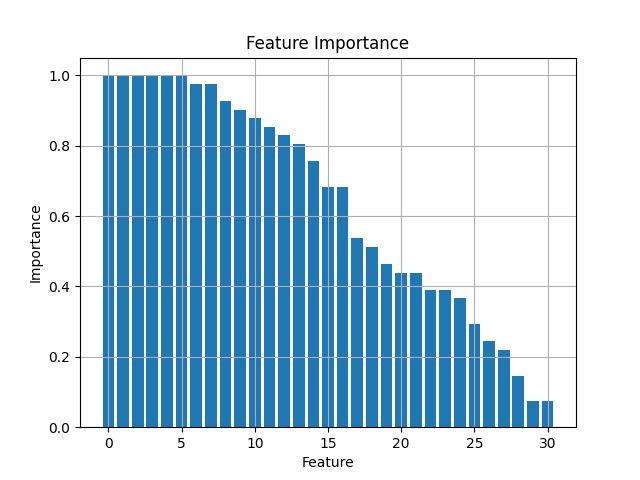
\includegraphics[scale=0.75]{images/feat_imp_barchart.jpg}
  \caption{Feature Importances}
  \centering
  \label{fig:fimp}
\end{figure}

The following are the features with importances above a threshold of 0.8.

\begin{table}[h!]
\centering
\begin{tabular}{|l|c|}
\hline
et0 fao evapotranspiration   &  1.0  \\ \hline
snow depth                   &  1.0  \\ \hline
diffuse radiation            &  1.0  \\ \hline
is day                       &  1.0  \\ \hline
relative humidity 2m         &  1.0  \\ \hline
terrestrial radiation        &  1.0  \\ \hline
temperature 2m               &  0.975  \\ \hline
soil temperature 0 to 7cm    &  0.975  \\ \hline
shortwave radiation          &  0.926  \\ \hline
sunshine duration            &  0.902  \\ \hline
wind direction 10m           &  0.878  \\ \hline
pressure msl                 &  0.853  \\ \hline
surface pressure             &  0.829  \\ \hline
cloud cover mid              &  0.804  \\ \hline

\end{tabular}
\caption{Most significant feature importances}
\label{tab:Top_fint}
\end{table}

Most of them are self-explanatory, and we will quickly explain the ones that are not:
\begin{itemize}
  \item \textbf{ET0 FAO56 EvapoTranspiration} is a composite irrigation indicator calculated using temperature, wind speed, humidity and solar radiation
  \item \textbf{Diffuse Radiation} is the amount of solar radiation reflected from particles in the air.
  \item \textbf{Terrestrial Radiation} is the amount of solar radiation that is reflected from the earth.
  \item \textbf{Shortwave radiation} is the amount of specific solar radiation with wavelengths in and around the visible spectrum.
  \item \textbf{Pressure MSL} represents the atmospheric pressure at the mean sea level
  \item \textbf{Cloud Cover Mid} is cloud coverage between 2km and 6km high
\end{itemize}

\subsection{Obtained models}

To compare the models using feature selection, we trained 3 preliminary models using LSTM model combined with static features. For comparison, we decided to use LSTMs with 1, 2 and 3 layers. The number of hidden neurons is the same for the static layer and the LSTM hidden layer which is 64.

Tables 2 and 3 summarize the performance evaluation of different model configurations. Among standalone LSTM models, the 2-layer architecture achieved the lowest RMSE on both test data (0.4094) and validation data (0.5153), slightly outperforming the 1-layer model and substantially outperforming the 3-layer variant.

The Random Forest meta-learner delivered the best test RMSE (0.3755) in ensemble setups, outperforming all standalone LSTM configurations. Conversely, the Single-Layer Perceptron (SLP) meta-learner exhibited poor generalization, with test and validation RMSEs exceeding 2.5.

However, when examining the RMSE values on the validation set, it becomes evident that models without feature selection perform better. This behaviour may be attributed to overfitting in the models with feature selection or suboptimal hyperparameter choices. Another plausible explanation is that the feature masks generated by the NSGA-II algorithm are not optimal, possibly due to insufficient evolutionary search. Increasing the number of generations or population size during optimization could improve the quality of the selected feature subsets.

\begin{table}[h]
\centering
\begin{tabular}{|l|l|}
\hline
Model            & RMSE       \\ \hline
LSTM 1 layer     & 0.42044225 \\ \hline
LSTM 2 layers    & 0.40944701 \\ \hline
LSTM 3 layers    & 0.46743059 \\ \hline
RF meta learner  & 0.37546269 \\ \hline
SLP meta learner & 2.55220830 \\ \hline
\end{tabular}
\caption{Root mean square of the test data}
\end{table}

\begin{table}[h]
\centering
\begin{tabular}{|l|l|}
\hline
Model            & RMSE       \\ \hline
LSTM 1 layer     & 0.55202835 \\ \hline
LSTM 2 layers    & 0.51527398 \\ \hline
LSTM 3 layers    & 0.54297155 \\ \hline
RF meta learner  & 1.07313182 \\ \hline
SLP meta learner & 2.86349174 \\ \hline
\end{tabular}
\caption{Root mean square of the validation data}
\end{table}

We also plot the model's predictions alongside the ground truth values of the time series to evaluate how well the network is performing. A well-known issue in time series forecasting arises when the model is fed previous target values as inputs—this can lead it to simply predict the current value as the last ground truth. This behaviour and many other potential issues become apparent when visualizing the predictions against the actual data.

Visualizations in Figures 2 through 5 further confirm that LSTM models are generally consistent, and the RF ensemble effectively smooths and enhances prediction accuracy.

\begin{figure}[H]
\centering
\subcaptionbox{One layer LSTM}{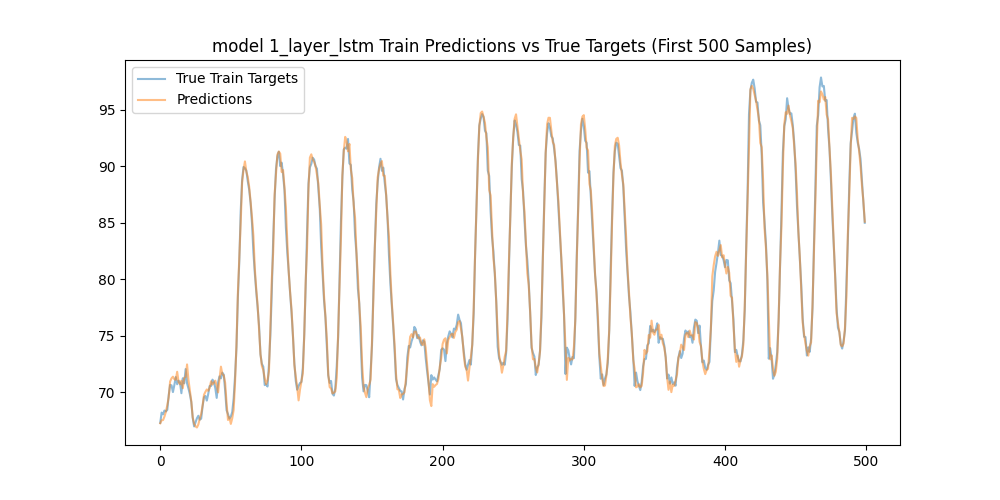
\includegraphics[width=0.50\textwidth]{results/plots/1_layer_lstm_train_predictions.png}}%
\hfill % <-- Seperation
\subcaptionbox{Two layers LSTM}{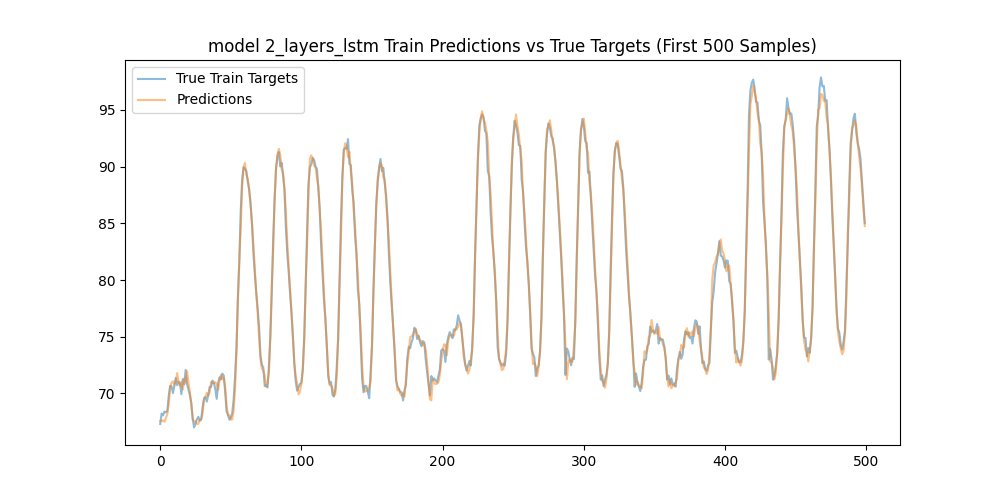
\includegraphics[width=0.50\textwidth]{results/plots/2_layers_lstm_train_predictions.png}}%
\hfill % <-- Seperation
\subcaptionbox{Three layers LSTM}{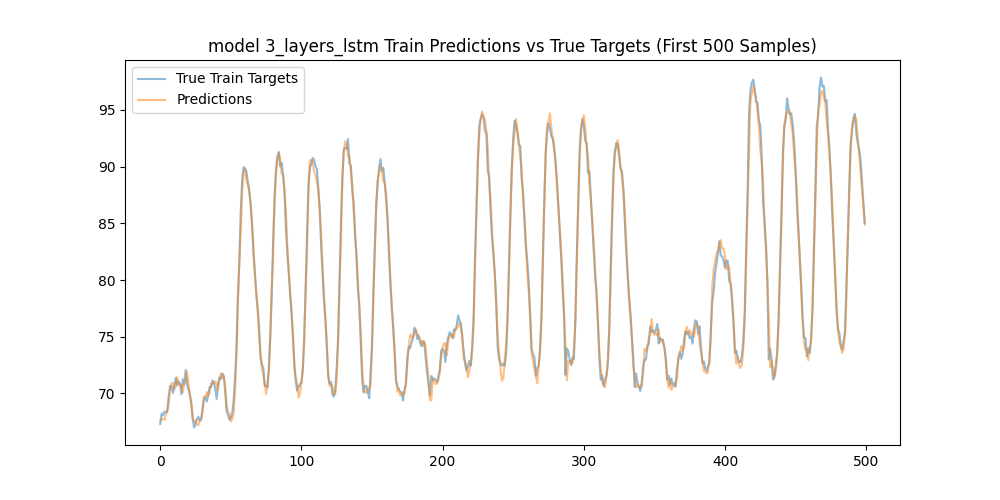
\includegraphics[width=0.50\textwidth]{results/plots/3_layers_lstm_train_predictions.png}}%
\caption{Train prediction for non feature selection models}
\end{figure}

\begin{figure}[H]
\centering
\subcaptionbox{Meta learner with random forest}{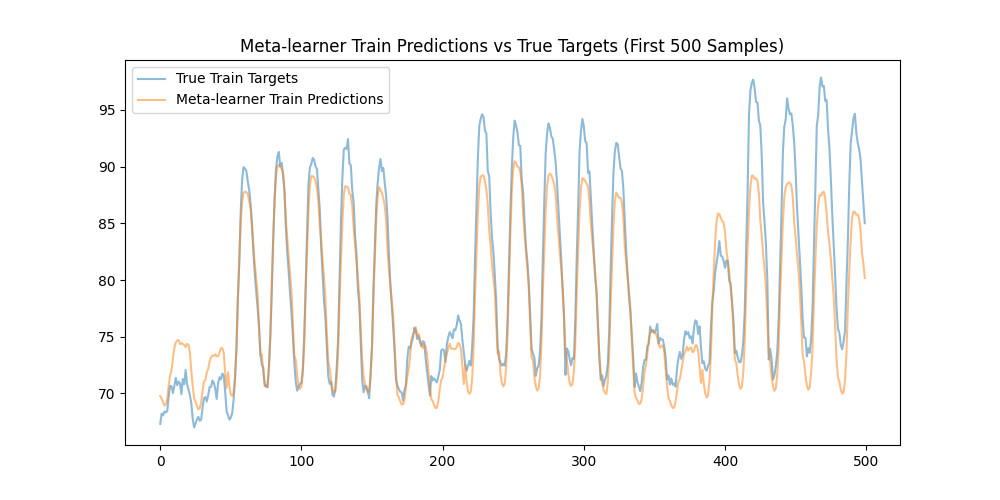
\includegraphics[width=0.50\textwidth]{results/plots/meta_learner_train_predictions.png}}%
\hfill % <-- Seperation
\subcaptionbox{Meta learner with SLP}{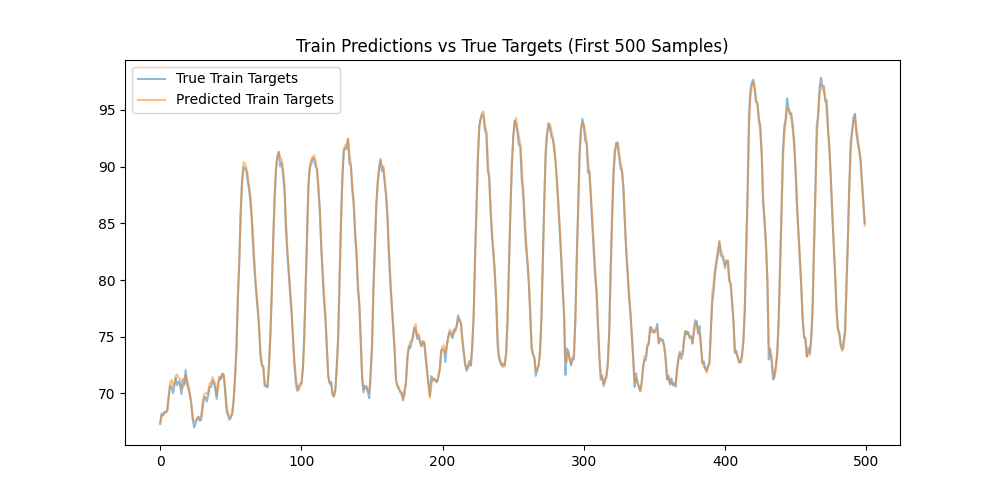
\includegraphics[width=0.50\textwidth]{results/plots/rf_train_predictions.png}}%
\caption{Train prediction for models with feature selection}
\end{figure}

\begin{figure}[H]
\centering
\subcaptionbox{One layer LSTM}{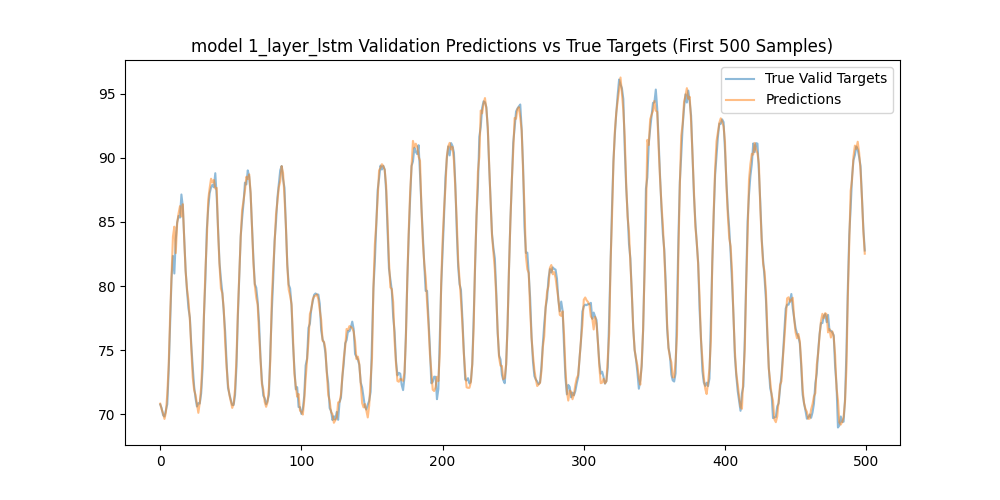
\includegraphics[width=0.50\textwidth]{results/plots/1_layer_lstm_valid_predictions.png}}%
\hfill % <-- Seperation
\subcaptionbox{Two layers LSTM}{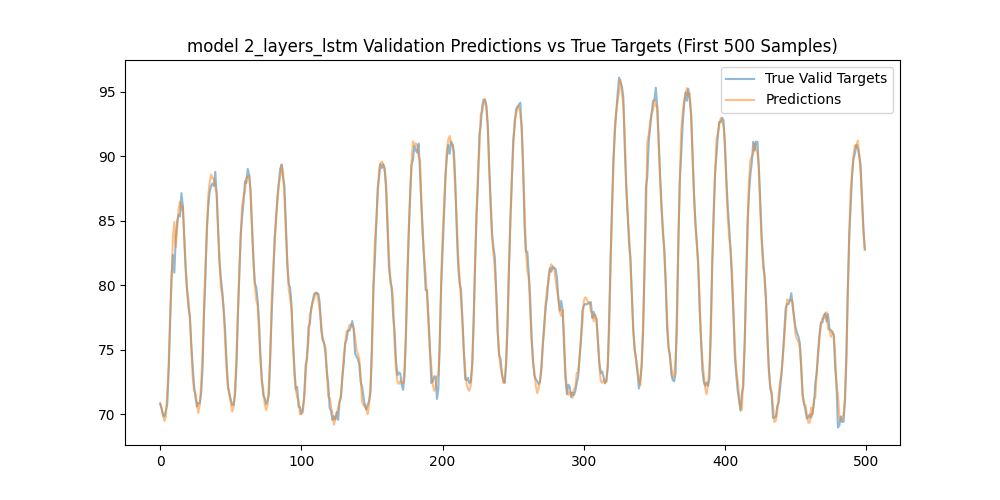
\includegraphics[width=0.50\textwidth]{results/plots/2_layers_lstm_valid_predictions.png}}%
\hfill % <-- Seperation
\subcaptionbox{Three layers LSTM}{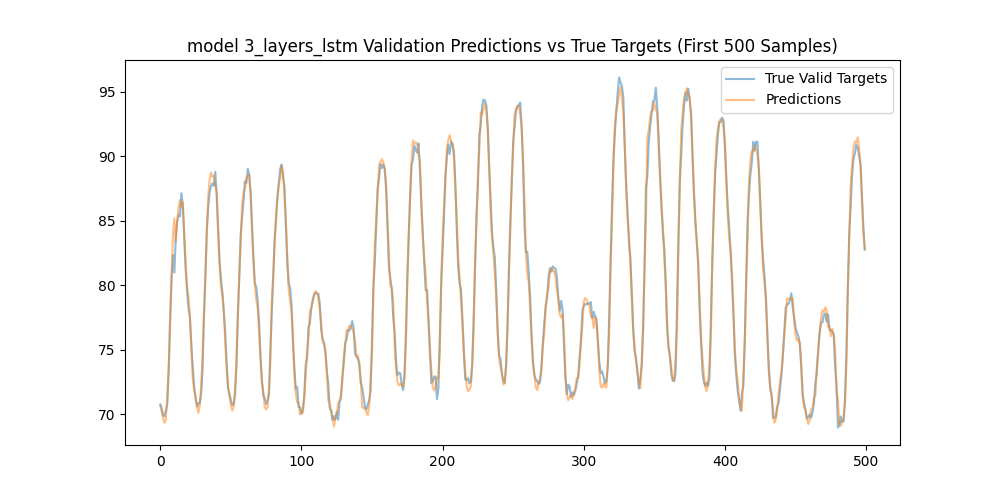
\includegraphics[width=0.50\textwidth]{results/plots/3_layers_lstm_valid_predictions.png}}%
\caption{Validation data prediction for non feature selection models}
\end{figure}

\begin{figure}[H]
\centering
\subcaptionbox{Meta learner with random forest}{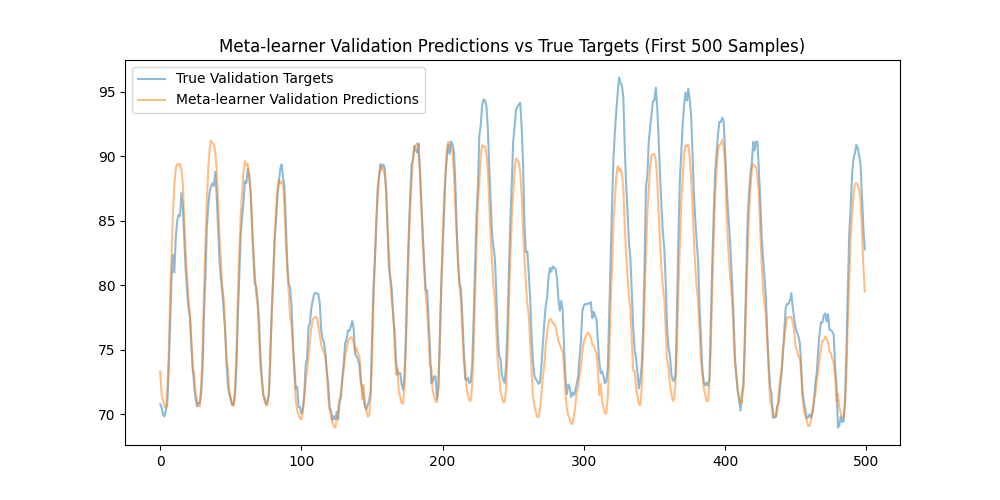
\includegraphics[width=0.50\textwidth]{results/plots/meta_learner_valid_predictions.png}}%
\hfill % <-- Seperation
\subcaptionbox{Meta learner with SLP}{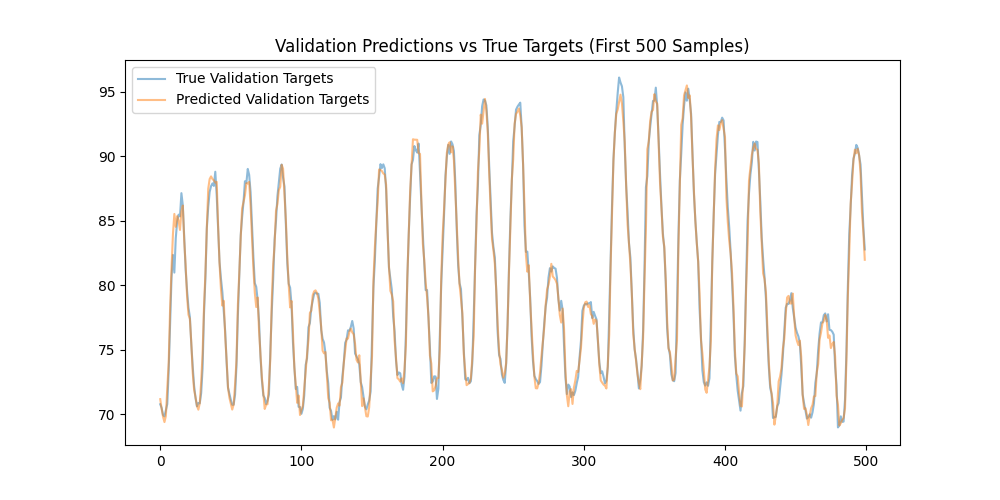
\includegraphics[width=0.50\textwidth]{results/plots/rf_valid_predictions.png}}%
\caption{Validation data prediction for models with feature selection}
\end{figure}

\section{Discussion}

In our feature analysis, we see that several features are present in all 45 of our partitions i.e. objective functions. They correspond to values of \textbf{1.0}. Nonetheless, we decided to keep all features with importance above \textbf{0.8}, which resulted in keeping \textbf{45\%} of our initial features. Additional preprocessing steps that consider correlation and other factors could further reduce this number while improving the results.

Based on the given importance, we can draw several conclusions. There exists a significant difference in electricity demand during daytime and nighttime. This can be attributed to the increase in human activity during the day, while most people are awake. Most of the shown features (sunshine, different radiations) are related to temperature, so that high and low temperatures incur cooling and heating, respectively. This is the biggest electricity demand factor, as almost half of the electricity in an (American) household goes into cooling and heating\footnote{\url{https://greenlogic.com/blog/the-top-5-biggest-users-of-electricity-in-your-home}}. Other features, such as cloud cover, relative humidity, wind direction and air pressure also have a large influence on the weather, and therefore temperature as well as our perception of it. While further analysis could give a deeper insight into the effects that these factors have on the electricity consumption, with our limited knowledge on the subject, we attribute most of it to temperature as the driving factor of electricity consumption.

The clear performance improvement of the RF meta-learner suggests that ensemble approaches can effectively combine diverse model behaviors and reduce individual biases. On the other hand, the poor performance of the SLP meta-learner indicates that model choice in ensemble learning is critical, especially when aggregating outputs from structurally diverse LSTM models.

The 2-layer LSTM model outperformed both the simpler and deeper versions, suggesting a balance between expressiveness and overfitting risk. The underperformance of the 3-layer model may be attributed to increased complexity and limited training data.

Computational demands also limited the number of evolutionary generations and population diversity, which may have impacted convergence. Simplified LSTM architectures were used to maintain feasibility, potentially reducing the model's ability to capture complex temporal patterns.

Nonetheless, the successful application of multi-objective optimization and ensemble learning under these constraints demonstrates the framework’s potential for interpretable and robust forecasting in real-world time series applications.

\section{Future Works}

Several directions can further improve our approach:

\begin{itemize}
    \item Increase NSGA-II Population: Expanding the population size and number of generations may yield better feature masks by enabling a more thorough search of the solution space.

    \item Remove Static Layer: Comparing models with and without the static input layer will clarify the true contribution of temporal context features like hour and day.

    \item Use Attention-Based LSTM \cite{Zhang_2019}: Introducing attention mechanisms can help directly visualize and interpret feature importance through learned weights.

    \item Study Hyperparameter Impact: Investigating how LSTM hyperparameters (e.g., number of layers, hidden size) affect mask selection could improve the integration of architecture tuning with feature selection.
\end{itemize}



\printbibliography

\end{document}

